\section{Cactus Environment Calculus} \label{sec:calc}

This section shows how the shared environment approach can be applied to
call by need evaluation. We start with a calculus with environments that can be
represented in either a shared or flat manner: Curien's calculus of closures,
and show how it can be modified to force sharing. See Curien's call by name
calculus of closures in Figure~\ref{fig:calcclos}\footnote{Curien calls it a
``lazy'' evaluator, and there is some ambiguity with the term lazy, but we use the
term only to mean call by need. We also remove the condition checking that $i <
m$ because we are only concerned with the evaluation of closed terms.}.

The LEval rule pushes a closure onto the environment, and the LVar rule indexes
into the environment, entering the corresponding closure. We show in this
section that by removing ambiguity about how the environments are represented,
and forcing them to be represented in a \emph{cactus stack}, we can define our
novel call by need calculus.

\begin{figure}
\textbf{Syntax}
\begin{align*}
\tag{Term} t &::= i \; | \; \lambda t \; | \; t \; t  \\
\tag{Variable} i &\in \mathbb{N}  \\
\tag{Closure} c &::= t [\rho] \\
\tag{Environment} \rho &::= \bullet \; | \; c \cdot \rho \\
\end{align*}
\textbf{Semantics}
\begin{align*}
\tag{LEval}\inference
{t_1[\rho] {\xrightarrow{* }}_L \lambda t_2[\rho'] }
{t_1 t_3[\rho] \rightarrow_L t_2[t_3[\rho] \cdot \rho'] } 
\end{align*}
\begin{align*}
\tag{LVar1} 0[c \cdot \rho] \rightarrow_L c
\end{align*}
\begin{align*}
\tag{LVar2} \inference
{i > 0}
{i[c \cdot \rho] \rightarrow_L (i-1)[\rho]}
\end{align*}
\caption{Curien's call by name calculus of closures}
\label{fig:calcclos}
\end{figure}

To start, consider again the example from Section~\ref{sec:env}, this
time with deBruijn indices: $(\lambda(\lambda t) \; (\lambda t_1)) t_2$.  The
terms $t$ and $t_1$ when evaluated in the closure calculus, would have the
following environments, respectively: 

\begin{center}
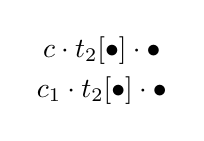
\begin{tikzpicture}
\node {$c \cdot t_2[\bullet] \cdot \bullet$};
\node [yshift=-0.5cm] {$c_1 \cdot t_2[\bullet] \cdot \bullet$};
\end{tikzpicture}
\end{center}

Again, the second closure in each environment is the same closure.  And again,
we can represent these environments with a shared environment, this time,
keeping call by need evaluation in mind:
\begin{center}
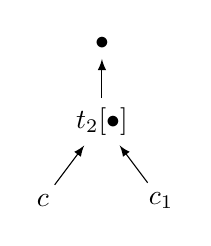
\begin{tikzpicture}[ 
  edge from parent path={(\tikzchildnode\tikzchildanchor) edge [-latex] (\tikzparentnode\tikzparentanchor)},
  level distance=1cm
]
\node (a) {$\bullet$} child{node (d) {$t_2[\bullet]$} child{node (b) {$c$}} child{node (c)
{$c_1$}}};

%\draw let \p1=(a), \p2 =(b), \n1={atan2(\y2-\y1,\x2-\x1)}, \n2={veclen(\y2-\y1,\x2-\x1)}
%  in ($ (a)!0.5!(b) $) ellipse [x radius=\n2/2+10pt, y radius=10pt, rotate=90-\n1];
%\draw let \p1=(a), \p2 =(c), \n1={atan2(\y2-\y1,\x2-\x1)}, \n2={veclen(\y2-\y1,\x2-\x1)}
%  in ($ (a)!0.5!(c) $) ellipse [x radius=\n2/2+10pt, y radius=10pt, rotate=90-\n1];
\end{tikzpicture}
\end{center}
This inverted tree structure seen earlier with the leaves pointing toward the
root is called a \emph{cactus stack} (sometimes called a spaghetti stack or
saguaro stack) \cite{hauck1968burroughs,ichbiah1979rationale}. In this
particular cactus stack, every node defines an environment as the sequence of
closures in the path to the root.  If $t_2[\bullet]$ is a thunk, and is updated
in place with the value after its first reference, then both environments would
contain the resulting value. This is exactly the kind of sharing that is
required by call by need, and thus we can use this structure to build a call by
need evaluator. This is the essence of the idea behind the cactus environment
calculus and the cactus environment ($\mathcal{CE}$) machine. Our important
insight here is that Curien's calculus of closures does not differentiate
between flat and shared environment representations, and indeed, no calculus
that we are aware of has had the need to.

Therefore, we must derive our own calculus of closures, forcing the environment
to be shared. Because we can hold the closure directly in the environment, we
choose to replace the standard heap of closures with a \emph{heap of
environments}. Because sharing is required, we extend Curien's calculus of
closures to include our heap of environments, or what we will refer to as a
\emph{cactus environment}. 

See Figure~\ref{fig:calccact} for the syntax and semantics of the cactus
calculus. Recall that we are only concerned with evaluation of closed terms. The
initial closed term $t$ is placed in a $(t[0],\epsilon[0=\bullet])$ tuple, and
evaluation terminates on a value. We define two different semantics, one for
call by name and one for call by need. This is to make the connection to
Curien's call by name calculus more straightfoward, both for the reader and
for the proof. The rule for application (MEval and NEval) is identical for
both semantics: each evaluates the left hand side to a function, then binds
the variable in the cactus environment, extending the current environment.
The only difference between this semantics and Curien's is that if we need
to extend an environment multiple times, the semantics \emph{require}
that we share said environment among the extensions. This makes no real
difference for call by name, but it is needed for the sharing of results in the
NVar1 rule. The explicit environment sharing ensures that the closure that is
overwritten with a value is shared between instances of that variable. 

\begin{figure*}
\textbf{Syntax}
\begin{align*}
\tag{Term} t &::= i \; | \; \lambda t \; | \; t \; t  \\
\tag{Variable} i &\in \mathbb{N}  \\
\tag{Closure} c &::= t [l] \\
\tag{Value} v &::= \lambda t [l] \\
\tag{Heap} \mu &::= \epsilon \; | \; \mu [ l \mapsto \rho ] \\
\tag{Environment} \rho &::= \bullet \; | \; c \cdot l \\
\tag{Location} l,f &\in \mathbb{N}  \\
\tag{State} s &::= (c, \mu)
\end{align*}
\textbf{Call by Name Semantics}
\begin{align*}
\tag{MEval} \inference
{(t[l], \mu) \xrightarrow{* }_{M} (\lambda t_2[l'], \mu') \quad f \not \in \textnormal{dom}(\mu')}
{(t \; t_3[l], \mu) \rightarrow_{M} (t_2[f], \mu'[f \mapsto t_3[l] \cdot l'])}  
\end{align*}
\begin{align*}
\tag{MVar1} \inference 
{\mu(l) = c \cdot l'}
{(0[l],\mu) \rightarrow_M (c,\mu)}
\end{align*}
\begin{align*}
\tag{MVar2} \inference
{i > 0 \quad \mu(l) = c \cdot l'}
{(i[l],\mu) \rightarrow_M ((i-1)[l'],\mu)}
\end{align*}
\textbf{Call by Need Semantics}
\begin{align*}
\tag{NEval} \inference
{(t[l], \mu) \xrightarrow{* }_{N} (\lambda t_2[l'], \mu') \quad f \not \in \textnormal{dom}(\mu')}
{(t \; t_3[l], \mu) \rightarrow_{N} (t_2[f], \mu'[f \mapsto t_3[l] \cdot l'])}  
\end{align*}
\begin{align*}
\tag{NVar1} \inference
{\mu(l) = c \cdot l' \quad (c, \mu) \xrightarrow{* }_{N} (v, \mu')}
{(0[l],\mu) \rightarrow_N (v, \mu'[l \mapsto v \cdot l'])}
\end{align*}
\begin{align*}
\tag{NVar2} \inference
{i > 0 \quad \mu(l) = c \cdot l'}
{(i[l],\mu) \rightarrow_N ((i-1)[l'], \mu)}
\end{align*}
\caption{Cactus calculus syntax and semantics.}
\label{fig:calccact}
\end{figure*}

\subsection{Correctness}

We use this section to show correctness with respect to Ariola et. al's call by
need lambda calculus \cite{ariola1995call}. In particular, we show correctness
with respect to their natural semantics (their Figure 8). 

\begin{figure}
\begin{align*}
\tag{Id} \inference
{\langle \Phi \rangle t \Downarrow \langle \Psi \rangle \lambda x.t'}
{\langle \Phi, x \mapsto t, \Upsilon \rangle x \Downarrow \langle \Psi, x
\mapsto \lambda x.t', \Upsilon \rangle \lambda x.t'}
\end{align*}
\begin{align*}
\tag{Abs} \inference 
{}
{\langle \Phi \rangle \lambda x . t \Downarrow \langle \Phi \rangle \lambda x.t}
\end{align*}
\begin{align*}
\tag{App} \inference
{\langle \Phi \rangle t_l \Downarrow \langle \Psi \rangle \lambda 
x.t_n \\ \langle \Psi, x' \mapsto t_m \rangle [x'/x]t_n \Downarrow \langle
\Upsilon \rangle \lambda y.t'}
{\langle \Phi \rangle t_l \; t_m \Downarrow \langle \Upsilon \rangle \lambda y.t'}
\end{align*}
\caption{Ariola et. al's Operational Semantics}
\label{fig:calccact}
\end{figure}

To start, case-wise induction on $\rightarrow_{N}$ gives us an ordering to the
closures in the cactus environment. This is similar to the ordering from Lemma
8.1 of \cite{ariola1995call}.

{\lemma $\forall_{l \mapsto t[l_1] \cdot l_2 \in \mu} l_1 < l \wedge l_2 < l$}
\vspace{2mm}

With this ordering, we can define a $flatten$ function that takes any $(c, \mu)$
and flattens it accordingly. It does so by mapping any $(c, \mu)$ to a $\langle
\Phi \rangle t$, with the necessary variable hygiene. With this function, along
with structural induction on term size, we get the following correctness
property:

{\prop \textnormal{(Correctness)} $(c, \mu) \xrightarrow{* }_{M} (v, \mu') \iff$
$$flatten(c,\mu) \Downarrow flatten(v, \mu') $$}

It is worth noting the similarity between these semantics for pedagogical
purposes. Ariola et. al's semantics throws out environmental structure because
it doesn't need to keep it. Indeed, keeping the structure would make
correspondence to their syntactic account more difficult. This is apparent in
how the abstract machines implementing the semantics (e.g.
\cite{garcia2009lazy}) are forced to do variable search in the environment:
deBruijn indices are not an option. Our machine, by retaining that structure in
the cactus environment, allows for use of deBruijn indices, and, as we will see
in Section~\ref{sec:impl}, straighforward low-level implementation.

\subsection{Recursion}

Correct sharing for recursive data values, as pointed out in
\cite{ariola1995call}, is not possible without adding explicit recursion. We
return to this issue in Section~\ref{sec:disc}, but at least mention here that
adding explicit recursion to this scheme would make for interesting future work.
